\section{Method of Regularized Stokeslets}
\subsection{Stokes flow}
When we look at many physical systems, particularly in biology, we find that the inertial forces within the fluid are small in comparison to that of the viscous terms. In these cases we can take the limit of the Navier-Stokes equation (\cref{eq:NavierStokes})where $R e=\rho u L/\mu \to 0 $ \cite{Trombley2019BasicFlows}. Within biological systems, we find that these cases occur when we are either looking at highly viscous fluids where $\mu$ is large or at small length scales where $L$ (The typical scale of the system) is very small such as when looking at cells, microorganism or flows around small capillaries \cite{Blake1972AOrganisms, Higdon1979APropulsion, Smith2009MathematicalFluids}. As well as biological models we can use it in more general fluid dynamics, where we have stokes flow, with complex boundaries \cite{Liron1978StokesPipe, Liron1976StokesPlates}.

The steady-state Stokes equations in two or three dimensions are
\begin{subequations}
\label{eq:StokesFlow}
\begin{align}
    \mu\Delta\boldsymbol{u} &= \nabla p - \boldsymbol{F} \label{eq:StokesFlow1} \\
    \nabla \cdot \boldsymbol{u} &= 0 \label{eq:StokesFlow2}
\end{align}
\end{subequations}
where $\mathbf{u}$ is the velocity of the fluid, $\mathbf{F}$ is the external body force, $p$ is the pressure and $\mu$ is the fluid viscosity.
We can derive a singular fundamental solution to the Stokes equations which we will call a \textit{Stokeslet}. The Stokeslet represents a solution for the velocity of the fluid given that an external force $\mathbf{F}$ acts on the fluid at a single point $\mathbf{F} = \mathbf{f_0}\delta(\mathbf{x})$ \cite{Hancock1953TheLiquids, Batchelor2000AnDynamics, Pozrikidis1992BoundaryFlow}.
Through similar methods to those shown later for deriving the regularized Stokeslet Equation (\cref{eq:regstokeslet2}) we can derive the singular fundamental solutions to the Stokes equations as
\begin{equation}
\label{eq:singularsolutions}
\begin{aligned}
    S_{j k}(\mathbf{x}, \mathbf{x_0}) &= \frac{\delta_{j k}}{r}+\frac{\left(x_{j}-x_{0,j}\right)\left(x_{k}-x_{0,k}\right)}{r^{3}} \\
    P_{k}(\mathbf{x}, \mathbf{x_0}) &= \frac{x_{k}-x_{0,k}}{r^{3}} \\
    T_{ijk}(\mathbf{x}, \mathbf{x_0}) &= \frac{-6\left(x_{i}-x_{0,i}\right)\left(x_{j}-x_{0,j}\right)\left(x_{k}-x_{0,k}\right)}{r^5}
\end{aligned}
\end{equation}
Where $r=|\mathbf{x}-\mathbf{x_0}|$. We can then find the velocity $\mathbf{u}$ at a point $\mathbf{x}$ through the equation
\begin{equation*}
    \mathbf{u} = (8 \pi \mu)^{-1} \left(S_{1j},S_{2j},S_{3j}\right)f_{0,j}
\end{equation*}
where $\mathbf{f_{0}}$ is the force per unit area exerted by the fluid on the surface, concentrated at the point $\mathbf{x_0}$.


\subsection{Regularising the Stokeslet}
While the singular Stokeslet provides a useful mechanism to solve boundary integral equations, it relies on the surfaces on which the Stokeslets are concentrated to be smooth such that the velocity is integrable and the fluid is bounded in the neighbourhood of the surface. However, if we consider non-smooth surfaces or curves instead then the resulting equations for velocity can become non-singular and much harder so work with.

\begin{figure}
    \centering
    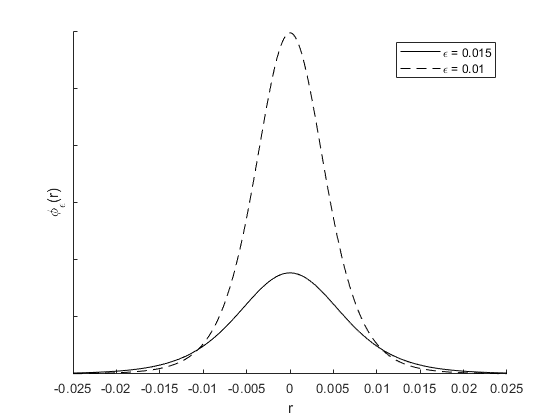
\includegraphics[scale=0.5]{Images/BlobFunction.png}
    \caption{Blob function in equation \cref{eq:blobfunc} for several values of epsilon}
    \label{fig:blobfunc}
\end{figure}

In order to remove these singularities, we use a cutoff/blob function which instead of approximating at force at a singular point we instead approximate as a sphere centred at the same point. While the radius of the sphere is often infinite the blob function decays rapidly away from the centre with the largest contribution obtained in the close vicinity of the centre. We introduce a control parameter $\epsilon$ independent of any discretization to control the rate of decay of the function. The effect of this control parameter can be seen in Fig.\cref{fig:blobfunc}. In order to obtain similar results to that of the singular solutions, we dictate that $\int \phi^\epsilon(r)dr=1$ for all values of $\epsilon$. This allows us to preserve the results obtained for the singular kernels for distances away from the point in which the force is exerted and obtain different results close to the point. In order to retain the singular solution, we have the condition that as $\epsilon \to 0$ our blob function must tend to the Dirac delta. For simplicity of the paper and the application to a wider range of problems, we will only consider spherically symmetric functions such as those in \cref{eq:blobfunc,eq:blobfunc2} \cite{Cortez2005,Olson2013ModelingFormulation,Nguyen2014ReductionFlow}.

\begin{align}
    \phi^\epsilon(r) &= \frac{15 \epsilon^4}{8\pi\left( r^2 +\epsilon^2 \right)^{7/2}} \label{eq:blobfunc}\\
    \phi_{\epsilon}(r) &= \frac{15 \epsilon^{6}\left(5-\frac{2 r^{2}}{\epsilon^{2}}\right)}{16 \pi\left(r^{2}+\epsilon^{2}\right)^{9 / 2}} \quad\quad \phi_{\epsilon}(r)=\frac{5 \epsilon^{2}-2 r^{2}}{2 \pi^{3 / 2} \epsilon^{5}} e^{-r^{2} / \epsilon^{2}} \label{eq:blobfunc2} 
\end{align}

For the derivation of the regularized Stokeslets and all further numerical analysis, we will use \cref{eq:blobfunc} due to its popularity in external literature and the simplicity of the kernel it generates.

\subsubsection{Derivation of the Regularized Stokeslet}
By concentrating the force onto a finite area using the blob function rather than a singular point as with the delta function. We therefore convert the stokes equations given in \cref{eq:StokesFlow} to a new set of regularised equations for which we will derive a set of solutions,
\begin{subequations}
\label{eq:RegStokesFlow}
\begin{align}
    \mu\Delta\boldsymbol{u} &= \nabla p - \phi^{\epsilon}(\mathbf{x}-\mathbf{x_0})\mathbf{f_0} \label{eq:RegStokesFlow1} \\
    \nabla \cdot \boldsymbol{u} &= 0 \label{eq:RegStokesFlow2}
\end{align}
\end{subequations}
where $f_0$ is the force per unit area as defined in the previous section.
In order to simplify notation from this point onwards, we will use the Einstein summation convention where repeated indices are summed over. We introduce the regularized Stokeslet function $S^\epsilon(\mathbf{x},\mathbf{x_0})$ which is the Green's function for the velocity $u^\epsilon(\mathbf{x})$. We can now write the solution to \cref{eq:RegStokesFlow} as
\begin{equation}
\label{eq:regvelsol}
    u_i(\mathbf{x}) = \frac{1}{8\pi\mu}S^\epsilon_{ij}(\mathbf{x},\mathbf{x_0})f_{0,j}
\end{equation}
The pressure and stress tensor associated with this flow can now be written as
\begin{gather}
\label{eq:regpressuresol}
    p(\mathbf{x}) = \frac{1}{8\pi}P^\epsilon_{j}(\mathbf{x},\mathbf{x_0})f_{0,j}\\
\label{eq:regstresssol}
    \sigma_{ik}(\mathbf{x}) = \frac{1}{8\pi}T^\epsilon_{ijk}(\mathbf{x},\mathbf{x_0})f_{0,j}\\
\end{gather}
By substituting these solutions back into \cref{eq:RegStokesFlow1} we find that they must obey
\begin{equation}
\label{eq:regcondition1}
    \Delta S^\epsilon_{kj}(\mathbf{x},\mathbf{x_0}) = \frac{\partial P^\epsilon_{j}(\mathbf{x},\mathbf{x_0})}{\partial x_k} - 8\pi\delta_{kj}\phi^\epsilon(\mathbf{x}-\mathbf{x_0})
\end{equation}
for all j and k with $\delta_{kj}$ being the Kronecker delta function. The impressibility condition \cref{eq:RegStokesFlow2} also gives us that
\begin{equation}
\label{eq:regcondition2}
    \frac{\partial S^\epsilon_{ij}(\mathbf{x},\mathbf{x_0})}{\partial x_i} = 0
\end{equation}
for all j. We next take the derivative of \cref{eq:regcondition1} with respect to $x_k$ to get
\begin{equation*}
    \frac{\partial S^\epsilon_{kj}(\mathbf{x},\mathbf{x_0})}{\partial x_i \partial x_i \partial x_k} = \frac{\partial^2 P^\epsilon_{j}(\mathbf{x},\mathbf{x_0})}{\partial x_k^2} - 8\pi\delta_{kj}\frac{\partial \phi^\epsilon(\mathbf{x}-\mathbf{x_0})}{\partial x_k}
\end{equation*}
Summing over $k$ as per the convention and using \cref{eq:regcondition2} gives us
\begin{equation}
\label{eq:regpressureeq}
    \Delta P^\epsilon_{j}(\mathbf{x},\mathbf{x_0}) = 8\pi\frac{\partial \phi^\epsilon(\mathbf{x}-\mathbf{x_0})}{\partial x_j}.
\end{equation}
If we now introduce the following two equations for algebraic simplicity
\begin{subequations}
\label{eq:intermediate}
\begin{align}
    \Delta G^\epsilon(\mathbf{x}-\mathbf{x_0})  &= \phi^\epsilon(\mathbf{x}-\mathbf{x_0}) \label{eq:inter1} \\
    \Delta B^\epsilon(\mathbf{x}-\mathbf{x_0})  &= G^\epsilon(\mathbf{x}-\mathbf{x_0}) \label{eq:inter2}
\end{align}
\end{subequations}
Using \cref{eq:inter1,eq:regpressureeq} we can express the pressure as
\begin{equation}
\label{eq:pressuresol}
    P^\epsilon_{j}(\mathbf{x},\mathbf{x_0})f_{0,j} = 8 \pi \frac{\partial G^\epsilon(\mathbf{x}-\mathbf{x_0})}{\partial x_j}
\end{equation}
Then finally using \cref{eq:regcondition1,eq:inter2} gives us the general for of our Stokeslet.
\begin{equation}
\label{eq:regstokeslet1}
    S_{ij}^\epsilon(\mathbf{x}, \mathbf{x_0}) = 8\pi\left[ \frac{\partial^2 B^\epsilon(\mathbf{x} -\mathbf{x_0})}{\partial x_i \partial x_j} - \delta_{ij}  G^\epsilon(\mathbf{x} -\mathbf{x_0})\right]
\end{equation}
As the stress tensor is defined as
\begin{equation}
\label{eq:regstress}
    \sigma_{ij}^\epsilon(\mathbf{x}) = -\delta_{ik}p^\epsilon(\mathbf{x}) + \mu\left( \frac{\partial u^\epsilon_i}{\partial x_k} + \frac{\partial u^\epsilon_k}{\partial x_i} \right)
\end{equation}
we find that
\begin{equation}
\label{eq:regDoubleLayerSol}
    T^\epsilon_{ijk}(\mathbf{x},\mathbf{x_0}) = -\delta_{ik} P^\epsilon_j(\mathbf{x},\mathbf{x_0}) + \mu\left( \frac{\partial S^\epsilon_{ij}(\mathbf{x},\mathbf{x_0})}{\partial x_k} + \frac{\partial S^\epsilon_{kj}(\mathbf{x},\mathbf{x_0})}{\partial x_i}\right)
\end{equation}

\subsubsection{Specific Blob}
If we take the blob equation defined in \cref{eq:blobfunc} and solve to find $G^\varepsilon$ and $B^\varepsilon$ we get that
\begin{subequations}
\begin{align}
    G^\varepsilon(\mathbf{x}-\mathbf{x_0}) &= \frac{-2r^2+3\epsilon^2}{8\pi(r^2+\epsilon^2)^{3/2}} + \frac{3}{8\pi\epsilon} \label{eq:G}\\
    B^\varepsilon(\mathbf{x}-\mathbf{x_0}) &= -\frac{\sqrt{\epsilon^2+r^2}}{8\pi} + \frac{r^2}{16\pi\epsilon} + \frac{\epsilon}{8\pi}\label{eq:B}
\end{align}
\end{subequations}
where $r=|\mathbf{x}-\mathbf{x_0}|$. We now substitute \cref{eq:G,eq:B} into \cref{eq:pressuresol,eq:regstokeslet1,eq:regDoubleLayerSol} to obtain our final kernels which will be used for all further analysis.

\begin{subequations}
\begin{align}
    P_j^\epsilon(\mathbf{x}, \mathbf{x_0}) =& (x_j-x_{0,j})\frac{2r^2+5\epsilon^2}{(r^2+\epsilon^2)^{5/2}} \label{eq:pressuresol2}\\
    S_{ij}^\epsilon(\mathbf{x}, \mathbf{x_0}) =& \delta_{ij} \frac{r^2+2\epsilon^2}{\left( r^2 + \epsilon^2 \right)^{3/2}} + \frac{(x_i-x_{0i})(x_j-x_{0j})}{\left( r^2 + \epsilon^2 \right)^{3/2}} \label{eq:regstokeslet2} \\
    T_{ijk}^\epsilon(\mathbf{x}, \mathbf{x_0}) =& \frac{-6(x_i-x_{0,i})(x_j-x_{0,j})(x_k-x_{0,k})}{(r^2+\epsilon^2)^{5/2}} \label{eq:doublelayer2}\\
    &-\frac{3\epsilon^2[\delta_{jk}(x_i-x_{0,i}) +\delta_{ik}(x_j-x_{0,j})+\delta_{ij}(x_k-x_{0,k})]}{(r^2+\epsilon^2)^{5/2}} \nonumber
\end{align}
\end{subequations}
We can easily check that these provide results consistent with those found by the singular solutions as in the limit $\epsilon \to 0$ we obtain the same results stated in \cref{eq:singularsolutions}.

\subsubsection{Boundary integral equations}

The solution to stokes equations
\begin{equation}
    \label{eq:BIE1}
\begin{aligned}
      \mu\Delta\boldsymbol{u} &= \nabla p \\
      \nabla \cdot \boldsymbol{u} &= 0
\end{aligned}
\end{equation}
and regularized Stokes equation
\begin{equation}
    \label{eq:BIE2}
\begin{aligned}
      \mu\Delta\boldsymbol{u} &= \nabla p - \phi_{\epsilon}(\mathbf{x}-\mathbf{x_0})\mathbf{f_0} \\
      \nabla \cdot \boldsymbol{u} &= 0
\end{aligned}
\end{equation}

are linked through the cutoff function and obtain the same results in the limit as $\epsilon \to 0$. It is assumed that the regularized solution is a flow generated by a point force of strength $\mathbf{f_0}$ located at a point $\mathbf{x_0}$ while the non-regularized solution is absent of all forces.

We let D be a solid body and assume the point $\mathbf{x}$ is outside of D. Then we have that ($\mathbf{u},p$) satisfies \cref{eq:BIE1} with
\begin{equation*}
\sigma_{ij}(\mathbf{x}) = -\delta_{ik}p(\mathbf{x}) + \mu\left( \frac{\partial u_i}{\partial x_k} + \frac{\partial u_k}{\partial x_i} \right)
\end{equation*}
and ($\mathbf{u^\epsilon},p$) satisfies \cref{eq:BIE2} with
\begin{equation*}
\sigma^\epsilon_{ij}(\mathbf{x}) = -\delta_{ik}p^\epsilon(\mathbf{x}) + \mu\left( \frac{\partial u^\epsilon_i}{\partial x_k} + \frac{\partial u^\epsilon_k}{\partial x_i} \right)
\end{equation*}
We note that $\partial \sigma_{ik}(\mathbf{x})/ \partial x_k = 0$ and $\partial \sigma^\epsilon_{ik}(\mathbf{x})/ \partial x_k = -f_{0_i}\phi^\epsilon(\mathbf{x}-\mathbf{x_0})$ through the use of \cref{eq:BIE1,eq:BIE2} respectively. From these two equations we find that
\begin{equation*}
\begin{aligned}
  \frac{\partial}{\partial x_k}(u^\epsilon_i\sigma_{ik} - u_i\sigma^\epsilon_{ik}) &=
  \frac{\partial u^\epsilon_i}{\partial x_k} \sigma_{ik} + u^\epsilon_i\frac{\partial \sigma_{ik}}{\partial x_k} - \frac{\partial u_i}{\partial x_k} \sigma^\epsilon_{ik} - u_i\frac{\partial \sigma^\epsilon_{ik}}{\partial x_k}  \\
  & = - u_i(-f_{0,i})\phi^\epsilon  \\
  &= u_j f_{0,j}\phi^\epsilon(\mathbf{x}-\mathbf{x_0})
\end{aligned}
\end{equation*}
where we have replaced the summation over $i$ with a summation over $j$ without affecting the result.
We now substitute in \cref{eq:regstresssol,eq:regvelsol} to obtain
\begin{equation*}
  \frac{1}{8\pi\mu}\frac{\partial}{\partial x_k}(S^\epsilon_{ij}f_{0,j}\sigma_{ik} - \mu u_i T^\epsilon_{ijk}f_{0,j}) = u_j f_{0,j}\phi_\epsilon(\mathbf{x}-\mathbf{x_0})
\end{equation*}
as $f_{0,j}$ is constant we can take it out of the derivative on the left-hand side and note that it is now arbitrary and as such $\mathbf{u}$ and $p$ obey the relation
\begin{equation}
  \label{eq:reciprocalrelation}
  \frac{1}{8\pi\mu}\frac{\partial}{\partial x_k}(S^\epsilon_{ij}\sigma_{ik} - \mu u_i T^\epsilon_{ijk}) = u_j\phi_\epsilon(\mathbf{x}-\mathbf{x_0})
\end{equation}
Suppose we now let $S$ be the area between the solid body $D$ and a sphere with a radius such that all of $D$ is contained within. We will denote $\partial S$ to be the surface of $S$, note that this contains the surface of the sphere and the surface of the solid body $\partial D$. If we now integrate the above equation over the volume $S$ then we get that
\begin{equation*}
  \int_{S} \left[\frac{1}{8\pi\mu}\frac{\partial}{\partial x_k}(S^\epsilon_{ij}\left(\mathbf{x}, \mathbf{x}_{0}\right)\sigma_{ik}\left(\mathbf{x}, \mathbf{x}_{0}\right) - \mu u_i(\mathbf{x}) T^\epsilon_{ijk}\left(\mathbf{x}, \mathbf{x}_{0}\right))\right] dV(\mathbf{x}) = \int_{S} u_j(\mathbf{x})\phi_\epsilon(\mathbf{x}-\mathbf{x_0}) dV(\mathbf{x})
\end{equation*}
Using the divergence theorem on the Left-hand side of the equation we get that
\begin{equation*}
  \frac{1}{8\pi\mu}\int_{\partial S} \left[S^\epsilon_{ij}\left(\mathbf{x}, \mathbf{x}_{0}\right)\sigma_{ik}\left(\mathbf{x}, \mathbf{x}_{0}\right) - \mu u_i(\mathbf{x} T^\epsilon_{ijk}\left(\mathbf{x}, \mathbf{x}_{0}\right)\right]n_k ds(\mathbf{x}) = \int_{S} u_j\phi_\epsilon(\mathbf{x}-\mathbf{x_0}) dV(\mathbf{x})
\end{equation*}
where $\mathbf{n}$ is the outwards unit normal vector of $\partial S$. If we consider the limit as the radius of the sphere tends to infinity, we find that the only contributions to the left-hand side come from $\partial D$. We will introduce the traction on the surface of the sphere as $f_i = -\sigma_{ik}n_k$ and obtain
\begin{equation}
\begin{aligned}
    \label{eq:BIE3}
    &\frac{1}{8\pi\mu}\int_{\partial D} S^\epsilon_{ij}\left(\mathbf{x}, \mathbf{x}_{0}\right)f_i(\mathbf{x}) ds(\mathbf{x}) - \frac{1}{8\pi}\int_{\partial D} u_i(\mathbf{x}) T^\epsilon_{ijk}\left(\mathbf{x}, \mathbf{x}_{0}\right)n_k(\mathbf{x}) ds(\mathbf{x}) \\
    &= \int_{S} u_j(\mathbf{x})\phi_\epsilon(\mathbf{x}-\mathbf{x_0}) dV(\mathbf{x})
\end{aligned}
\end{equation}

Considering the fluid inside of the solid body $D$ we realise that the velocity must satisfy the zero-deformation condition
\begin{equation*}
  \frac{\partial u_i}{\partial k} + \frac{\partial u_k}{\partial i} = 0
\end{equation*}
This gives us that $\sigma_{ik} = -p\delta_{ik}$ inside of $D$ and as such we obtain that for each $j=1,2,3$
\begin{equation*}
  \int_{D} \frac{\partial}{\partial x_k}\left[S^\epsilon_{ij}\left(\mathbf{x}, \mathbf{x}_{0}\right)\sigma_{ik}\left(\mathbf{x}, \mathbf{x}_{0}\right)\right]dV(\mathbf{x}) = -p\int_{D} \frac{\partial}{\partial x_k}\left[S^\epsilon_{kj}\left(\mathbf{x}, \mathbf{x}_{0}\right)\right]dV(\mathbf{x}) = 0
\end{equation*}
from the incompressibility condition \cref{eq:regcondition2}. If we now integrate \cref{eq:reciprocalrelation} over $D$ instead of $S$ and use the above integral we have that given $p \neq 0$
\begin{equation}
\begin{aligned}
      \label{eq:BIE4}
-\frac{1}{8\pi}\int_{D} \frac{\partial}{\partial x_k}\left(u_i(\mathbf{x})T^\epsilon_{ijk}\left(\mathbf{x}, \mathbf{x}_{0}\right) \right) dV(\mathbf{x}) &= \frac{1}{8\pi}\int_{\partial D} u_i(\mathbf{x})T^\epsilon_{ijk}\left(\mathbf{x}, \mathbf{x}_{0}\right)n_k(\mathbf{x}) ds(\mathbf{x})\\
&= \int_D u_j(\mathbf{x}) \phi^\epsilon(\mathbf{x}-\mathbf{x_0}) dV(\mathbf{x})
\end{aligned}
\end{equation}
We again have used the divergence theorem to convert the volume integral to a surface integral with $n_k$ being defined to point into $D$. Observing that the sum over \cref{eq:BIE3,eq:BIE4} will give us the integral over $\mathbb{R}^{3}$ and using the fact that the velocity is continuous on the boundary $\partial D$ we obtain the final boundary integral equation is
\begin{equation}
  \label{eq:BIE5}
    \int_{\mathbb{R}^{3}} u_{j}(\mathbf{x}) \phi^{\epsilon}\left(\mathbf{x}-\mathbf{x}_{0}\right) d V(\mathbf{x})=-\frac{1}{8 \pi \mu} \int_{\partial D} S_{i j}^{\epsilon}\left(\mathbf{x}, \mathbf{x}_{0}\right) f_{i}(\mathbf{x}) d s(\mathbf{x})
\end{equation}
As the traction $\mathbf{f}$ denotes the force exerted by the fluid on the body it must have the opposite sign to the Stokeslet strength $\mathbf{f_0}$ and as such $\mathbf{f_0} = -\mathbf{f}$. In order to use \cref{eq:BIE5} we need to have an explicit equation for $\mathbf{u}(\mathbf{x})$, as such we need to remove the integral and the cutoff function from the left hand side of \cref{eq:BIE5}, we do this though the approximation that $\int_{\mathbb{R}^{3}} u_{j}(\mathbf{x}) \phi^{\epsilon}\left(\mathbf{x}-\mathbf{x}_{0}\right) d V(\mathbf{x}) \approx u_j(\mathbf{x_0})$. By taking the approximation as exact we write that 
\begin{equation}
    u_j(\mathbf{x_0}) = \frac{1}{8 \pi \mu} \int_{\partial D} S_{i j}^{\epsilon}\left(\mathbf{x}, \mathbf{x}_{0}\right) f_{0,i}(\mathbf{x}) d s(\mathbf{x})
\end{equation}
By using the fact that $S_{i j}^{\epsilon}\left(\mathbf{x}, \mathbf{x}_{0}\right) = S_{j i}^{\epsilon}\left(\mathbf{x}_{0}, \mathbf{x}\right)$ we can write \cref{eq:BIE5} as 
\begin{equation}
  \label{eq:BIE}
    u(\mathbf{x})_i=\frac{1}{8 \pi \mu} \int_{\partial D} S_{i j}^{\epsilon}\left(\mathbf{x}, \mathbf{x}_{0}\right) f_{0,j}(\mathbf{x_0}) d s(\mathbf{x_0})
\end{equation}
The analysis of this error for our particular cutoff function can be see in \cite{Cortez2005} and is found to be of order $\mathcal{O}(\epsilon)$ close to the boundary and $\mathcal{O}(\epsilon^2)$ away from the boundary.


The analytical computation of \cref{eq:BIE} is possible for certain cases allowing for the computation of the fluid velocity given prescribed body forces on the fluid, however, they are often hard or impossible to do by hand. In this case we consider the numerical integration of such problems. By approximating the boundary integral equation with a quadrature rule ${\mathbf{x}_0}_n A_n$ we obtain a formula for the velocity of the fluid at a point $\mathbf{x_0}$. To do this we consider the integral on the right-hand side of \cref{eq:BIE} as the sum over N Stokeslets located along the surface of $D$. 
\begin{equation}
\label{eq:Stokesletsum}
    u_{i}\left(\mathbf{x}\right)=\frac{1}{8 \pi \mu} \sum_{n=1}^{N} \sum_{i=1}^{3} S_{i j}^{\epsilon}\left(\mathbf{x}, {\mathbf{x}_0}_{n}\right) {f_0}_{n, j} A_{n}
\end{equation}
where ${f_0}_{n, i}$ is the $i$th component of the force on the fluid at ${\mathbf{x}_0}_n$ and $A_n$ is the corresponding quadrature weight of the $n$th Stokeslet. 

It is often more common that we wish to compute the velocity at a set of collocation points $\{\mathbf{x_n}\}$. We note that as long as we keep the quadrature rule the same for all collocation points then we keep the set of ${f_0}_{n, i}$ remains the same and only $\mathbf{x}$ changes for each collocation point. The implies that the computation of this sum can for a single collocation point be viewed as the product of a dense $3 \times 3N$ matrix with a $3N \times 1$ column vector where N is the number of Stokelets. By extension of this idea the computation for a set of collocation points can be viewed as the product of a dense $3M \times 3N$ matrix with a $3N \times 1$ column vector where $M$ is the number of collocation points in which we wish to compute the velocity at.  
The computation of this matrix vector product can be written as 
\begin{equation}
\label{eq:matrixvectorproduct}
    U = A \cdot F
\end{equation}
where $U$ is a $3M \times 1$ column vector, $A$ is a $3M \times 3N$ matrix and $F$ is a $3N \times 1$. In order to form an equation of this form we choose to write 
\small
\begin{equation*}
    U = [u_1(x_{0,1}), \; u_2(x_{0,1}), \; u_3(x_{0,}), \; u_1(x_{0,2}), \; u_2(x_{0,2}), \; u_3(x_{0,2}), \; \dots \; u_1(x_{0,M}), \; u_2(x_{0,M}), \; u_3(x_{0,M})]^{T}
\end{equation*}
\normalsize
and 
\small
\begin{equation*}
    F = [f_{1,1}A_1, \; f_{1,2}A_1, \; f_{1,3}A_1, \; f_{2,1}A_2, \; f_{2,2}A_2, \; f_{2,3}A_2, \; \dots \; f_{N,1}A_N, \; f_{N,2}A_N, \; f_{N,3}A_N]^{T}
\end{equation*}
\normalsize
This gives the form of A as 
\small
\begin{equation*}
A = 
\begingroup
\setlength\arraycolsep{1pt}
\begin{bmatrix}
S^{\epsilon}_{1,1}(\mathbf{x}_1,\mathbf{x_{0}}_1) & S^{\epsilon}_{1,2}(\mathbf{x}_1,\mathbf{x_{0}}_1) & S^{\epsilon}_{1,3}(\mathbf{x}_1,\mathbf{x_{0}}_1) & \dots & S^{\epsilon}_{1,1}(\mathbf{x}_N,\mathbf{x_{0}}_1) & S^{\epsilon}_{1,3}(\mathbf{x}_N,\mathbf{x_{0}}_1) & S^{\epsilon}_{1,3}(\mathbf{x}_N,\mathbf{x_{0}}_1)\\
S^{\epsilon}_{2,1}(\mathbf{x}_1,\mathbf{x_{0}}_1) & S^{\epsilon}_{2,2}(\mathbf{x}_1,\mathbf{x_{0}}_1) & S^{\epsilon}_{2,3}(\mathbf{x}_1,\mathbf{x_{0}}_1) & \dots & S^{\epsilon}_{2,1}(\mathbf{x}_N,\mathbf{x_{0}}_1) & S^{\epsilon}_{2,2}(\mathbf{x}_N,\mathbf{x_{0}}_1) & S^{\epsilon}_{2,3}(\mathbf{x}_N,\mathbf{x_{0}}_1)\\
S^{\epsilon}_{3,1}(\mathbf{x}_1,\mathbf{x_{0}}_1) & S^{\epsilon}_{3,2}(\mathbf{x}_1,\mathbf{x_{0}}_1) & S^{\epsilon}_{3,3}(\mathbf{x}_1,\mathbf{x_{0}}_1) & \dots & S^{\epsilon}_{3,1}(\mathbf{x}_N,\mathbf{x_{0}}_1) & S^{\epsilon}_{3,2}(\mathbf{x}_N,\mathbf{x_{0}}_1) & S^{\epsilon}_{3,3}(\mathbf{x}_N,\mathbf{x_{0}}_1)\\
\vdots & \vdots & \vdots & \ddots & \vdots & \vdots & \vdots \\
S^{\epsilon}_{1,1}(\mathbf{x}_1,\mathbf{x_{0}}_M) & S^{\epsilon}_{1,2}(\mathbf{x}_1,\mathbf{x_{0}}_M) & S^{\epsilon}_{1,3}(\mathbf{x}_1,\mathbf{x_{0}}_M) & \dots & S^{\epsilon}_{1,1}(\mathbf{x}_N,\mathbf{x_{0}}_M) & S^{\epsilon}_{1,2}(\mathbf{x}_N,\mathbf{x_{0}}_M) & S^{\epsilon}_{1,3}(\mathbf{x}_N,\mathbf{x_{0}}_M)  \\
S^{\epsilon}_{2,1}(\mathbf{x}_1,\mathbf{x_{0}}_M) & S^{\epsilon}_{2,2}(\mathbf{x}_1,\mathbf{x_{0}}_M) & S^{\epsilon}_{2,3}(\mathbf{x}_1,\mathbf{x_{0}}_M) & \dots & S^{\epsilon}_{2,1}(\mathbf{x}_N,\mathbf{x_{0}}_M) & S^{\epsilon}_{2,2}(\mathbf{x}_N,\mathbf{x_{0}}_M) & S^{\epsilon}_{2,3}(\mathbf{x}_N,\mathbf{x_{0}}_M) \\
S^{\epsilon}_{3,1}(\mathbf{x}_1,\mathbf{x_{0}}_M) & S^{\epsilon}_{3,2}(\mathbf{x}_1,\mathbf{x_{0}}_M) & S^{\epsilon}_{3,3}(\mathbf{x}_1,\mathbf{x_{0}}_M) & \dots & S^{\epsilon}_{3,1}(\mathbf{x}_N,\mathbf{x_{0}}_M) & S^{\epsilon}_{3,2}(\mathbf{x}_N,\mathbf{x_{0}}_M) & S^{\epsilon}_{3,3}(\mathbf{x}_N,\mathbf{x_{0}}_M) \\
\end{bmatrix}
\endgroup
\end{equation*}
\normalsize

We will from now on refer to the computation of the velocities at the set of points $\{ \mathbf{x_{0,n}} \}$ through the direct computation of the full vector-matrix product as the direct solution.
We do note that this particular choose in the structure of $U$ and $F$ is not unique and other literature may use different arrangements however they will all produce the same results. 

By writing our system in this form it allows for easy implementation in software such as Matlab where we can make use of highly optimised BLAS (Basic Linear Algebra Subprograms) and LAPACK (Linear Algebra PACKage) packages over direct computations in the code. This allows for the software to use the latest in hardware and software optimisations such as improved multicore algorithms and across multiple types of hardware with no changes to the higher-level code.